% ===========================================================================
% v3 §3 — THE HARNESS, COMPONENT BY COMPONENT (replaces v2 §3 "The Agentic Workflow")
% Census commit for every count marked \prov: 4df6884 (roster T1, commit 427fdc5).
% Figure F1 = paper_agentic/figures/fig_F1_harness_anatomy (gated; sha d355cbec…).
% Table T1 = paper_agentic/v3/tab_T1_roster.tex (generated from the roster; appendix).
% v2 text that MOVES rather than dies: "Inside the fitting step" -> §4 (with F3);
% "Two planes" -> §6; "The doctrine" -> §5; the register + hierarchy paragraphs of
% "The operating skeleton" -> §5; the state/cascade paragraphs -> §3.4 below; the
% authority table -> §3.5 below. Nothing is cut without a later chng that shows where it went.
% ===========================================================================
\section{The Harness, Component by Component} \label{sec:harness}

We use one vocabulary throughout. The \emph{model} is the language model we
call; it reasons, and it has no memory between calls and no way to check
its own claims against the world. The \emph{harness} is everything around
that call that lets the system act and keeps it honest. Recent engineering
accounts of agent harnesses\footnote{Bowne-Anderson, ``How to build an
effective agent harness'' (2026); B\"ockeler, ``Harness engineering for
coding agent users'' (2026); the Palantir Ontology documentation; and two
vendor posts. URLs in the provenance manifest.} converge on five runtime
jobs: run the reasoning loop, execute tools, assemble and manage context,
persist state, and enforce boundaries. Figure~\ref{fig:anatomy} lays our
system out under those five jobs, drawing each component solid where it
exists on disk and dashed where it is only proposed. Table~\ref{tab:roster}
(Appendix~\ref{app:roster}) states the work of every component in one
sentence, with its origin quoted and dated. The counts in this section are
taken at one commit\prov{} and will move; the roster says which commit.

\begin{figure*}[t]
\centering
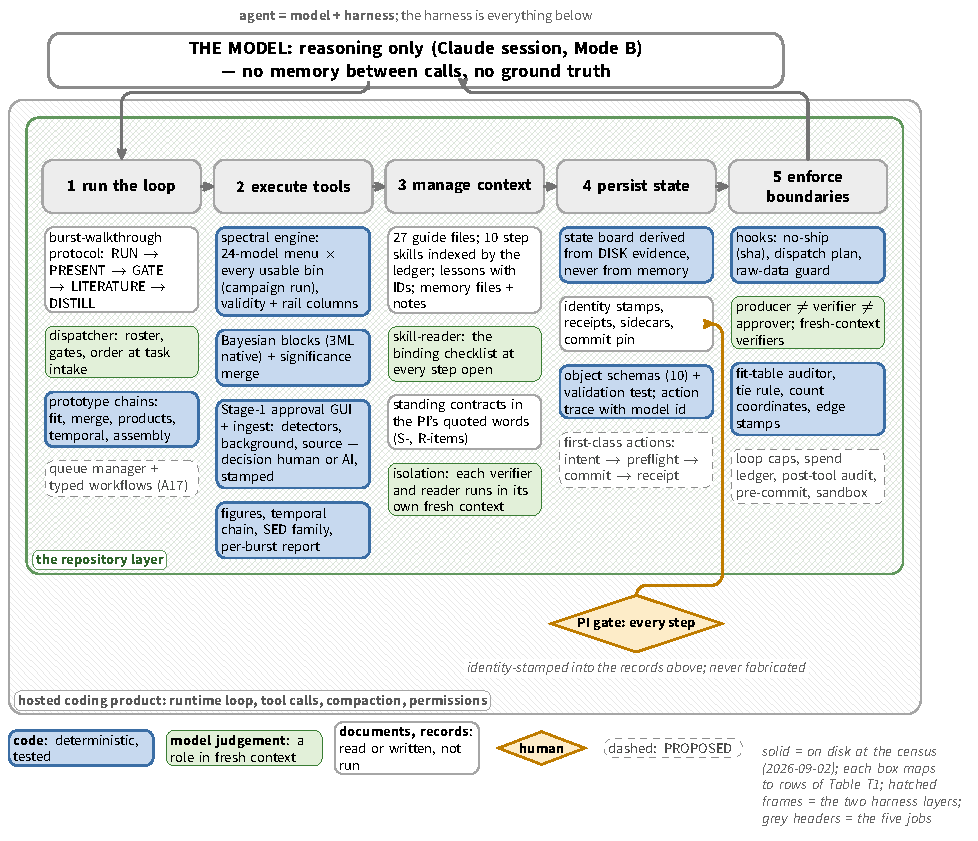
\includegraphics[width=\textwidth]{figures/fig_F1_harness_anatomy.pdf}
\caption{The harness anatomy. The five runtime jobs of an agent harness,
with the components this campaign has under each. Solid boxes exist on
disk at the census commit; dashed boxes are proposed in the requirements
register but not yet built. The human gate stamps every step with an
identity; approvals are never generated on the human's behalf. Each box
maps to rows of Table~\ref{tab:roster}.}
\label{fig:anatomy}
\end{figure*}

\subsection{The loop and the state machine} \label{sec:loop}

The reasoning loop today is the interactive session of a commercial coding
harness, which we call Mode~B: the harness supplies the loop, the tool
execution, the compaction of long context, and a permission layer, and our
repository supplies everything that makes the session a GRB analyst. The
per-burst protocol drives that loop: each of the eleven steps of the burst
ledger is run, presented to the human in a fixed four-sentence form, gated,
compared with the literature where the step calls for it, and distilled
before the next step starts. A \emph{dispatcher} reads each task and the
requirements register at intake and returns the agents, gates, and order the
task requires, naming every guard that does not yet exist. The loop is
stateful only through the disk: a burst occupies one of fourteen typed
states\prov{} (thirteen from ingested to closed, plus one terminal
exclusion), and the state is derived from the products on disk at read
time, never asserted by the session.

Two parts of the loop are declared debt. The queue manager that would own
campaign sequencing, hold the memory-budget claims, and resume after a
kill, and the eleven typed workflows\prov{} that would run each state
transition as a fixed sequence of reader, producers, verifiers, and stamps,
are specified in the skeleton document and not built; transitions run today
on prototype shell chains that invoke no agent. We draw both dashed and
return to what their absence costs in \S\ref{sec:discussion}.

\subsection{Tools: the deterministic producers} \label{sec:tools}

The tools are ordinary, testable code, and the agents command them through
a deliberately small interface: nine of the ten agent definitions carry only
file reading, searching, and a shell, and the tenth adds file editing so
that it can write lessons. The domain instruments are the spectral engine,
which fits twenty-four models\prov{} to every time bin and to the integrated
window and writes a validity flag, the bound-pinning diagnostics, and the
information criteria for each; the adaptive binning tool, which cuts the
brightest detector's light curve into Bayesian blocks and merges blocks
below a significance floor using the fitting library's own classes; the
Stage-1 approval tool, which shows the light curves and records a human or
vision-agent decision on detectors, background windows, and source window
with a stamp naming who approved and how; the temporal chain, which
measures durations, the minimum variability timescale, and the spectral
lag from the same approved selections and imports the lag routine we
validated in an earlier project unmodified; the spectral-energy panel
family, which renders each bin under the display semantics of the standard
X-ray fitting package and refuses any panel that disagrees with the stored
fit; and the report assembler, which writes one document per burst from
that burst's own numbers. The fitting step, where most of the bounded
agency lives, is described with its own figure in \S\ref{sec:sensors}.

\subsection{Context: skills, checklists, and memory} \label{sec:context}

Context is what the model sees when it acts, and the harness's job is to
give it the right context at every step without letting the accumulation of
a long run crowd out what matters. Three moves do this. \emph{Reduce}: the
harness compacts old conversation, and the per-burst live report is rebuilt
from stamps rather than carried in prose. \emph{Offload}: durable knowledge
lives in files the model reads on demand, chiefly twenty-seven skill
documents\prov{} indexed by the burst ledger, each carrying its criteria,
its checklist, and its numbered lessons with a prefix unique to the file,
and a small set of standing contracts written in the human's quoted words
for figures and reports. \emph{Isolate}: every verification runs in a fresh
context that has seen nothing of the producer's reasoning, and inventories
of the repository are delegated to agents that return conclusions rather
than file dumps. The \emph{skill reader} turns the offloaded law into
action: it opens every step by reading the step's skill document, its
defect ledger, and the open register rows, and returns the binding checklist
for \emph{this} burst. It produces nothing else. Cross-session memory is a
small indexed file of durable facts, read at the start of every session and
updated by a consolidation step, never trusted to recollection.

\subsection{State: derived from disk, stamped, receipted} \label{sec:state}

The system may claim only what it can evidence. Its state board is computed
from the files on disk for all one hundred and six bursts\prov, so the board
cannot say a step ran when its products are absent. Every step gate leaves
an approval stamp naming the approver, the time, and the status, and the
live report is assembled only from stamps and products it can link.
Approvals are revocable by machine: when an upstream decision is amended, a
cascade demotes every downstream approval that depended on it, and
reinstatement requires a human ruling with evidence. Both directions have
operated in production. The cascade exposed an approval that had been given
in conversation but never stamped, and the record carries it with the delay
disclosed rather than back-dated; a demoted binning approval was reinstated
only on proof that the binning's reference detector was untouched by the
amendment, its block table byte-identical\prov.

Products bind to their inputs by content hash and to their generators by
commit: a promotion receipt records the hash of the staged and promoted
tables, a sidecar beside every fit table records the detectors, ranges, and
convention in force, and a commit pin fixes the generator code for the
campaign. Since the census day, ten of the object types the pipeline
writes\prov{} carry a JSON schema, and a test validates every instance on
disk against it; the first run of that test found the literature-harvest
manifests spelling their paper list under four different keys and two
malformed bibliographic codes, which is what a schema is for. One honesty
item remains: products live in two roots resolved by an index file, so the
system does not yet have one reality; the object-and-action model of
\S\ref{sec:objects} says what closing that gap requires.

\subsection{Boundaries: hooks, roles, and the human gate} \label{sec:boundaries}

Boundaries are enforced at the strongest layer that can hold them. Three
repository hooks\prov{} act before a tool call runs: no figure reaches the
human unless its hash appears in a verification ledger; no pipeline
producer launches without a dispatch plan younger than a day; and raw data
cannot be deleted or overwritten by a shell command. Their limits are
stated as plainly as their powers. The no-ship hook sees only image files;
the dispatch hook covers one of the five pipeline transitions\prov{} and
matches the text of a command rather than what it executes, so it has
blocked read-only commands that merely named a producer; and the raw-data
guard is a pattern, not a filesystem jail. Everything the hooks do not
cover is enforced by fresh-context agents and, weakest of all, by prose.

Roles are separated by construction. The producer of an artifact never
verifies it, the verifier never approves it, and the approver is the human
at every step gate. Four kinds of actor appear in the action record: the
human, who approves and rules; the agent, whose identity and model are
stamped on what it presents, verifies, or distils; the hook, which refuses;
and the script, which produces and writes its receipt. The identity that
would approve in a fully automated mode is a decision the human has not yet
taken, and we list it as pending rather than assume it.

\begin{deluxetable*}{lll}
\tablecaption{The authority split: who decides what.\label{tab:authority}}
\tablehead{\colhead{the workflow decides (predefined)} & \colhead{the AI decides (bounded agency)} & \colhead{the human decides (gates)}}
\startdata
step order and Protocol & model winner via the gated comparison & scope and completion contract \\
energy selections; statistic & fit-validity verdicts & every Stage-1 selection (stamped) \\
multistart seeds; bound gates & literature verification and frame alignment & every step gate \\
provenance stamping & mismatch attribution; lesson drafting & lesson acceptance; convergence; freeze \\
typed terminal states & anomaly flagging and escalation & promotion from the discovery plane; every claim \\
\enddata
\end{deluxetable*}

Table~\ref{tab:authority} states the paper's honesty contract. The
\emph{workflow} decides everything decided in advance: the step order, the
energy selections, the statistic, the multistart seeds, the stamping of
provenance. The \emph{AI} decides, within audited bounds: which model wins
the gated comparison, whether a fit is valid, whether a published value has
been verified at source and in which frame, how a mismatch is attributed,
and which anomalies deserve escalation. The \emph{human} decides everything
consequential: the scope, every step gate, whether a proposed lesson enters
the library, when convergence is declared, and every scientific claim that
leaves the system. In all operation to date\prov, no approval has been
generated by the system on the human's behalf; the reverse, the human
overruling the agent's proposal, occurred repeatedly and is part of the
record (\S\ref{sec:discussion}).

What the roster makes visible, finally, is the shape of the harness as it
stands: forty-four of forty-nine components\prov{} exist on disk and five are
proposed, and the five that are missing are the ones that would turn
protocol into mechanism. The queue manager, the workflows, the
report-conformance gate, the first-class actions, and the loop caps are all
of that kind. We return to this pattern, and to what it says about where a
scientific harness should grow next, in \S\ref{sec:discussion}.
